\chapter{Methodology}
\label{chap:methodology}

\iffalse
The type of research you did
How you collected your data
How you analyzed your data
Any tools or materials you used in the research
Your rationale for choosing these methods

\begin{enumerate}
    \item What is the state of the art for real time event correlation?
    \item How can we improve the way real time event correlation is done for Windows Event Logs? %How can multi-threaded programming language and better rule formats improve how real time event...
    \item What is the performance of our proposed method, and how does it compare to other methods?
\end{enumerate}

\anders{Vil bare understreke at du kanskje er ute etter en vitenskapelig metode her, ikke å gå inn på hvorfor du valgte Go. Go er implmentasjonen din, mer på begrunnelse i en beskrivelse av valg av verktøy for performance reasons or whatnot. Når jeg leser methodology i en vitenskapelig oppgave/artikkel/avhandling så skal det gå på om du f.eks. utvikler noe nytt, bidrar til en felles forståelse om bedring av et eksisterende miljø eller noe sånt svada.}
\fi

The goal of this thesis is to explore.. if there is any way that we can improve the way real time event correlation is done, and in particular for Windows Event Logs.
In the chapter \cref{chap:background} we discussed the background and state of the art for doing event correlation.

\section{Datasets}
\label{sec:datasets}
To properly address the Research Questions proposed, it is important to have one or more datasets that can be used to evaluate the performance of the proposed solution in this thesis.
There is not a vast variety of available datasets that focus on Windows Event Logs publicly available, but there are some that have surfaced in the recent years. We will present those in the following section and offers a short evaluation in the context of this thesis.

\subsection{Evaluation of existing datasets}
\label{sub:evaluation-of-existing-datasets}
When evaluating which datasets we want to use for our experiments, we first have to define some parameters that we can measure the datasets by:
\begin{itemize}
    \item Size - The dataset must be large enough to measure the performance of existing solutions and our proposed solution.
    \item Representative - The dataset must be representative of the real world
    \item Up to date - The dataset should be of a recent date \todo{Because?}
\end{itemize}

\subsubsection{Boss of the SOC}
Boss of the SOC (BOTS) are datasets created for Splunks Boss of the SOC capture the flag competitions. The datasets are created in a controlled environment, where some adversary actions has been taken. The contestants have to analyze and hunt in the data to answer several security-related questions which grant points.

\todo{Describe the BOTS-datasets}
\todo{Run some actual tests against the dataset to see if we get a hit with our rules}

There are multiple versions of the BOTS datasets.
\textbf{Version 1}
\url{https://github.com/splunk/botsv1}

\todo{Acquire this dataset}

\textbf{Version 2}
\url{https://github.com/splunk/botsv2}

There are two versions; one which only contains attacker-related data, and one with the all the data, including noise. We have chosen to use the full dataset. This version contains a variety of different data sources. The one we are interested in is called xmlwineventlog. The dataset contains 1 093 753 lines of xmlwineventlog data. We have to convert this to our syslog-format, and we can simply do that using a Python script.


\textbf{Version 3}
\url{https://github.com/splunk/botsv3}

Contains 9 212 lines of xmlwineventlog events.

\subsubsection{Mordor}
\url{https://github.com/hunters-forge/mordor}
The Mordor datasets are pre-recorded events generated by simulating adversarial techniques in a test environment using common red team tools like Empire and Cobalt Strike. The largest dataset in the collection aims to simulate a Advanced Persistent Threat (APT) known as APT3/Gothic Panda. The dataset contains two scenarios, both outlined in MITRE ATT\&CK Evaluation Operational Flow. The flow maps directly to MITREs ATT\&CK framework, by stepping through 10 different "steps".

\begin{enumerate}
\item Initial Compromise
\item Initial Discovery
\item Privilege Escalation
\item Discovery for Lateral Movement
\item Credential Access
\item Lateral Movement
\item Persistence
\item Collection
\item Exfiltration
\item Execution of Persistence
\end{enumerate}

The dataset contains approximately 100 000 log lines, and is made for security analysts to test their skills and tools using real known bad data.

\subsubsection{EVTX-ATTACK-SAMPLES}
\url{https://github.com/sbousseaden/EVTX-ATTACK-SAMPLES/}

event log file (.evtx or .evt files) \textcite{windows_events_docs}

\subsubsection{Synthetic datasets}

\textbf{High signal, low noise dataset}\\
The concentrated dataset is a generated dataset that repeats the same 3 log lines that are enough to trigger a rule. The dataset is made in different sizes, from 1 000 lines, up to 1 million lines.

This dataset is in no way "realistic", and is only used for performance testing when evaluating our real-time analysis throughput in a "worst case"-scenario setting.

\textbf{Low signal, high noise dataset}\\
This is the opposite of the highly concentrated dataset which contained the necessary log lines to repeatedly trigger a specific rule. This dataset only contains the necessary events to trigger a single rule once, the rest of the events are simply background noise.

\textbf{Baseline dataset}\\
This dataset is a dataset with events that are all benign. This dataset is useful for measuring the speed at which the tools process and analyse the events, without triggering any rules.

\subsection{Dataset discussion}
\n{Are they realistic?}\\
\n{Are they represenative?}\\
\textbf{Concentrated dataset}\\
The concentrated dataset is used strictly for measuring the performance of the systems in a worst-case scenario, and the dataset is in itself not representative of a real world scenario, ingesting log data that doesn't contain malice.\\
\textbf{Mordor datasets}\\
The Mordor datasets are not as concentrated and gathered from a test environment using realistic tools, techniques and procedures based on the MITRE ATT\&CK framework.

\subsection{Datasets used in this thesis}
\label{sec:datasets-used}

For the experiments conducted in this thesis, Multiple datasets have been chosen:

\begin{itemize}
    \item Mordor dataset
    \item High signal, low noise dataset
    \item Low signal, high noise dataset
    \item Baseline dataset
\end{itemize}
The reason for choosing these datasets are many. First of all we chose the Mordor dataset as it is sufficiently large enough, representative and up-to-date. Then we have chosen the synthetic datasets as they will be used for baselining, best and worst-case scenarios for performance measuring.

\section{Improving real time event correlation for Windows Event Logs}
\label{sec:improving-real-time-event-correlation-for-windows-event-logs}

With regards to Research Question 2 in Section \cref{sec:researchquestions}, the question we are trying to answer is if there are ways we can improve how real time event correlation is done. Our approach should 

\subsection{Compiled language vs. interpreted language}
\label{sub:use-compiled-language}

Does a compiled programming language give us benefits in terms of performance, compared to an interpreted programming language?

\todo{Casually mention Go here?}

There are several reasons to use gravitate towards Go as the language of choice.
\begin{itemize}
    \item Compiled language offer performance benefits over interpreted languages
    \item Go routines and channels makes it easy to implement concurrent execution as discussed in Section \cref{sub:concurrent-execution}.
    \item Cross-platform
    \item Garbage collection
    \item Strongly and statically typed
    \item Race-condition detection
    \item Built-in profiling tools
\end{itemize}

\begin{figure}[htbp]
    \centering
    \begin{subfigure}[b]{.45\textwidth}
        \centering
        \begin{tikzpicture}[->,>=stealth',shorten >=1pt,auto, node distance=1.5cm, thick,
                    exe/.style={rectangle, minimum width=1cm, minimum height=1cm, rounded corners, text centered, draw=black, fill=red!30},
                    stepp/.style={rectangle, minimum width=1cm, minimum height=1cm,text centered, draw=black, fill=orange!30},
                    libraryy/.style={rectangle, rounded corners, minimum width=1cm, text centered, draw=black, fill=green!30}]
        \node (Source) [stepp] {Source};
        \node (Compilation) [libraryy, below of=Source] {Compilation};
        \node (Executable) [exe, below of=Compilation] {Executable};
        \node (Input) [stepp, left of=Executable, xshift=-1cm] {Input};
        \node (Output) [stepp, right of=Executable, xshift=1cm] {Output};
        
        \path[every node/.style={font=\sffamily\small}]
        (Source)
            edge node {} (Compilation)
        (Compilation)
            edge node {} (Executable)
        (Input)
            edge node {} (Executable)
        (Executable)
            edge node {} (Output)
        ;
        \end{tikzpicture}
        \caption{Compiled language model}
        \label{sfig:compiled-language}
    \end{subfigure}
    \hfill
    \begin{subfigure}[b]{.45\textwidth}
        \centering
        \begin{tikzpicture}[->,>=stealth',shorten >=1pt,auto, node distance=1.5cm, thick,
                    exe/.style={rectangle, minimum width=1cm, minimum height=1cm, rounded corners, text centered, draw=black, fill=red!30},
                    stepp/.style={rectangle, minimum width=1cm, minimum height=1cm,text centered, draw=black, fill=orange!30},
                    libraryy/.style={rectangle, rounded corners, minimum width=1cm, text centered, draw=black, fill=green!30}]
        \node (Source) [stepp] {Source};
        \node (Input) [stepp, right of=Source] {Input};
        \path (Source) -- (Input) coordinate[midway] (aux);
        \node (Interpreter) [libraryy, below of=aux] {Interpreter};
        \node (Output) [stepp, below of=Interpreter] {Output};
        
        \path[every node/.style={font=\sffamily\small}]
        (Source)
            edge node {} (Interpreter)
        (Input)
            edge node {} (Interpreter)
        (Interpreter)
            edge node {} (Output)
        ;
        \end{tikzpicture}
        \caption{Interpreted language model}
        \label{sfig:interpreted-language}
    \end{subfigure}
    \caption{Illustration of compiled vs. interpreted language}
    \label{fig:compiled-and-interpreted-language}
\end{figure}


\subsection{Concurrent execution}
\label{sub:concurrent-execution}

As seen with the existing solutions, they are not taking full advantage of the system when only running in a single thread. We believe that by using multi-threading we can increase the throughput of the solution and process events much quicker.

\begin{figure}[ht]
  \centering
\begin{ganttchart}[
    y unit title = 0.6cm, title height=1,
    vgrid={*1{draw=black!15, line width=.75pt}},
    hgrid,
]{1}{16}
  \gantttitlelist{1,...,16}{1} \\
  \ganttbar[bar/.append style={fill=red!50, rounded corners=3pt}]{Thread 1}{1}{2}
  \ganttbar[bar/.append style={fill=blue, rounded corners=3pt}]{}{3}{4}
  \ganttbar[bar/.append style={fill=red!50, rounded corners=3pt}]{}{5}{6}
  \ganttbar[bar/.append style={fill=blue, rounded corners=3pt}]{}{7}{8}
  \ganttbar[bar/.append style={fill=red!50, rounded corners=3pt}]{}{9}{10}
  \ganttbar[bar/.append style={fill=blue, rounded corners=3pt}]{}{11}{12}
  \ganttbar[bar/.append style={fill=red!50, rounded corners=3pt}]{}{13}{14}
  \ganttbar[bar/.append style={fill=blue, rounded corners=3pt}]{}{15}{16}
\end{ganttchart}
  \caption{Synchronously processing of 8 events}
  \label{gantt:synchronous-execution}
\end{figure}

\begin{figure}[ht]  %t top, b bottom, p page | you can also use h to try to get the figure to appear at the current location
  \centering
\begin{ganttchart}[
    y unit title = 0.6cm, title height=1,
    vgrid={*1{draw=black!15, line width=.75pt}},
    hgrid
]{1}{16}
  \gantttitlelist{1,...,16}{1} \\
  \ganttbar[bar/.append style={fill=red!50, rounded corners=3pt}]{Thread 1}{1}{2}
  \ganttbar[bar/.append style={fill=blue, rounded corners=3pt}]{}{3}{4} \\
  \ganttbar[bar/.append style={fill=blue, rounded corners=3pt}]{Thread 2}{1}{2}
  \ganttbar[bar/.append style={fill=red!50, rounded corners=3pt}]{}{3}{4}\\
  \ganttbar[bar/.append style={fill=red!50, rounded corners=3pt}]{Thread 3}{1}{2}
  \ganttbar[bar/.append style={fill=blue, rounded corners=3pt}]{}{3}{4}\\
  \ganttbar[bar/.append style={fill=blue, rounded corners=3pt}]{Thread 4}{1}{2}
  \ganttbar[bar/.append style={fill=red!50, rounded corners=3pt}]{}{3}{4}
\end{ganttchart}
  \caption{Concurrent processing of 8 events}
  \label{gantt:concurrent-execution}
\end{figure}


\subsection{Better rules}
\label{sub:better-rules}

By building the program in a different way, can we use other type of rules that perform better than the ones current seen?

As stated by \textcite{rouillard2004real}, the majority of the computational time used in \acrshort{sec} is spent on matching events against regular expression.

\subsection{Proper time management}
\label{sub:time-management}

Instead of the time being based on when the event is read, we want to base our correlation on when the event was generated by the system. This introduces several problems implementation-wise.

\subsection{Something something preprocessing of logs}

We propose that tokenization is a better option for handling certain types of logs. Move away from regular expressions and over to tokenization instead.

We are talking about tokenization in the lexical form, not data security.

\subsection{Support for multiple log formats}
\label{sub:multiple-log-formats}

Currently we are focused on Windows Event Logs, but the solution could be expanded into supporting other log sources without much work. We consider this future work.

\subsection{Output modularity}
\label{sub:modularity}

Defining different alert output channels. It would be nice to be able to create granular output rules that takes some decision based on the alert severity and sends the alert to the proper channel. Channels could include:

\begin{itemize}
    \item E-Mail
    \item Instant Messaging platforms like Slack, Teams et cetera.
    \item Ticketing system
    \item SIEM products like Splunk
\end{itemize}
We have chosen not to implement these as we focused primarily on performance measurements, and consider this future work.

\subsection{Distributed correlation}
\label{sub:distributed-correlation}

\begin{itemize}
    \item Geolocation - Reduce latency by ingesting data from hosts as close to them as possible
    \item Redundancy - If a ingestion node experiences issues
    \item Scalability - Architecture-wise we want to upscale...
\end{itemize}

\begin{figure}[ht]  %t top, b bottom, p page | you can also use h to try to get the figure to appear at the current location
  \centering
  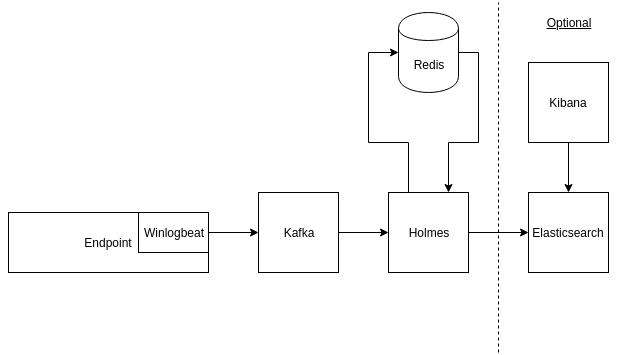
\includegraphics[width=.85\textwidth]{figures/holmes-architecture}
  \caption[An example figure.]{Minimal architecture. Every single node can be scaled both vertically and horizontally.}
  \label{fig:example}
\end{figure}
When scaling a system, we generally consider two different types of scaling. Horizontal and vertical. Horizontal scaling means that we are adding additional machines into a pool of resources for that particular service. Vertical scaling is adding more power to the existing machine, for instance by increasing the available RAM or upgrading the CPU(s).
There are multiple considerations that have to be done when choosing which way to scale a system. Horizontal scaling usually comes with the drawback of having to manage the pool of resources for each scaled service. Vertical scaling is in general simpler, but at some point it is no longer possible or feasible to scale further with regards to performance and cost.
The implementation show in this thesis is primarily built to scale vertically.
Interesting future work would be to add horizontal scaling to the proposed solution in this thesis, and tackle the challenges associated with load balancing, shared "context memory" between the correlators, and other possible obstacles.


\section{Measuring performance}
\label{sec:measuring-performance}
There are multiple factors that affect the performance of event correlators. All these factors lead to multiple ways that we can measure performance. This section tries to outline the most important ones.

\subsection{Hardware utilization}
\label{sub:hardware-utilization}
Another approach when 
Measuring RAM and CPU usage may show the most efficient, fastest, greenest solution.

\subsection{Data ingestion speed}
\label{sub:ingestion-speed}

At the start of the data pipeline, we have to ingest our data for processing. Data ingestion is the process of importing data from an external source into our program. The rate at which we are ingesting events are usually measured in events per second.
Data ingestion is based on a emitter sending the data, and a receiver receiving the data. The emitter does not have to be a separate system, it can be a hard disk, RAM or a network-based service. 
The performance related to data ingestion speeds can be bottlenecked by several possible things. The emitter may be bound by the storage medium it is sending data from. If we are reading events from a log file stored to disk, we are bound to the read speed that our disk(s) support. If we are reading events from a process that stores the events in memory, we are bound by the read speeds of our RAM.
With regards to network-based transmission, the choice of transport-layer protocol used can have an impact on transmission speed. Using UDP may be the fastest, but could lead to dropped packages which not optimal. Using TCP ensures that all events are transmitted, but at the cost of additional overhead for re-transmitting lost data, re-arranging packets out of order, et cetera. When transmitting data in a network (both internal and via the internet) encryption is needed to ensure authenticity and tamper protection of the data. But encryption comes at a cost, namely that it takes some time to encrypt and decrypt data when its sent and received.
Additionally, the networking hardware can play a role depending on the setup. The supported speeds of the network card in the emitter and receiver, and any intermediate networking equipment like switches and routers could affect the throughput of events.
There are multiple ways of transmitting data over the network that may affect the ingestion speed, and that is the implementation of how transmitting shall be done. Real-time transmission sends the events as soon as they happen, one-by-one. Another tactic is to use batching or chunking that sends bursts of events instead of sending the events one-by-one. Finally, a hybrid approach is possible where the emitter chooses which type to use depending how many events are being transmitted.
Then we have the ingestion capabilities of the receiver. This boils down to how efficient the receiver is to manage the backlog of events it receives. A simple program might only allow processing one event at the time, blocking incoming new events. A more efficient program might store a backlog of events in RAM, which ensures that it does not block incoming new events.

There are multiple ways we can measure all these different possible bottlenecks. For disk and RAM-based operations we can use profiling tools that come with the operating system to measure the load we are under. We can look at the number and size of the network packages being sent and received. Given an external emitter running for instance the software Kafka, we can get an overview of how fast receivers are fetching data from the emitter. Likewise, we can do the same from the end of the receiver by looking at how many events we are ingesting into our program per second. Finally, we can test the ingestion using timing, by ingesting a set number of events and timing how fast the receiver can ingest them (without any processing other than ingesting), we can calculate the number of events per second.

\subsection{Processing speed}
\label{subs:processing-speed}
Since the ingestion speed discussed in \cref{sub:ingestion-speed} might fluctuate depending on how the data is ingested, measuring the internal processing speed might be more interesting when evaluating the performance of the various solutions. This removes the uncertainties related to ingestion speeds. There are multiple options when looking at internal processing speed. One might look at the processing as a whole from start to finish, or try to separate out the various internal steps that occur during processing. Go features a profiler that will output a graph, showing which functions are taking up the most time during runtime. This can give an idea of where the most of the time is spent during processing.

The processing speed can be affected by several things. First of all the dataset used will matter, as the number of matches will have an effect on the number of alerts generated and contexts updated.
Secondly, the implementation of how rules are processed and checked against events can have a big impact on the processing speed. If the solution is able to quickly disregard events as not interesting, there is a big potential for saving time.
Lastly, the internal handling of contextual information, how that information is accessed and other performance-related improvements all have an effect on the processing speed observed.
% Drawback
The biggest drawback of this approach is the need profiling or timing "inside" the solution. While this might be simple to implement in a new solution, patching such a feature into older solutions can prove to be hard or in the worst case error-prone if the solution being patched is not fully understood.

\subsection{Compound processing speed}
\label{sub:compound-processing-speed}

Measuring the compound processing speed will give us a bird's-eye view of what the total processing speed is. It takes into account both ingestion and processing speeds, measures the total time used, including both I/O and any internal processing.

Depending on the solutions, this might be the best or only option for a good one-to-one comparision between solutions.


\section{Test plan}
As highlighted, there are multiple ways that we can improve or further expand the capabilities of existing real time event correlation solutions. In Chapter \cref{chap:experiments} we will focus on the improvements mentioned in Section \cref{sub:use-compiled-language}, \cref{sub:better-rules} and \cref{sub:time-management}. Distributed correlation, output modularity and support for multiple log formats as discussed in \cref{sub:distributed-correlation}, \cref{sub:modularity}, \cref{sub:multiple-log-formats} is future work.
As discussed in \cref{sec:measuring-performance}, there are multiple ways that we can measure the performance of our solution against existing solutions. We will primarily be using compound processing speed as discussed in \cref{sub:compound-processing-speed} for our performance tests.
\iffalse
\section{The Go programming language}

\com{Her er en rask intro, argumentasjonen hvorfor vi valgte dette finner du i eksperiment XYZ}
\todo{Why did we choose Go?} \com{Dette er ikke teori/bakgrunn, men mer et metodevalg.}
\subsection{Goroutines}
\todo{What are these lightweight Go threads?}\\
Goroutines are lightweight threads that are handled by the Go runtime.
\subsection{Channels}

\todo{What are channels? What are some of the considerations we have to take when working with them?}\\
\todo{Are there any best practices?}\\
Channels are the preferred way to communicate between Goroutines in Go.

\subsection{Concurrency vs parallelism}
\todo{Discuss why Go is concurrent, but not parallel}
\fi